\documentclass{beamer}

\mode<presentation> {

\usepackage{graphicx}
\usepackage[utf8]{inputenc}
\usepackage[ngerman]{babel}
\usepackage[outputdir=output]{minted} % Syntax-Highlighted Code; requires pygments to be installed

\usetheme{Boadilla}
\usecolortheme{seagull}

\setbeamertemplate{footline}[page number] % Einfacher Folienzähler als Fußzeile
\setbeamertemplate{navigation symbols}{} % Keine Navigationslinks
}

\defbeamertemplate*{title page}{customized}[1][]
{
  \centering
  \usebeamerfont{title}{\LARGE \inserttitle}\par
  \usebeamerfont{subtitle}\usebeamercolor[fg]{subtitle}\insertsubtitle\par
  \bigskip
  \usebeamercolor[fg]{titlegraphic}\inserttitlegraphic\par
  \bigskip
  \usebeamerfont{author}\insertauthor\\[0.5em]
  \usebeamerfont{institute}\insertinstitute\par
  \usebeamerfont{date}\insertdate\par
}

\title[Lens]{Lenses und Zauberwürfel}
\titlegraphic{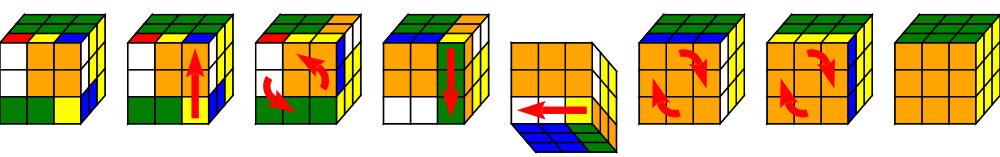
\includegraphics[width=0.65\linewidth]{rubiks-sequence.png}}
\author{Tim Baumann}
\institute[CCA]{Curry Club Augsburg}
\date{13. August 2015}

\newcommand{\kreuz}{$\,^\dag$} % Dagger, alter!
\newcommand{\kkreuz}{$\,^\ddag$} % DDagger, alter!
\newcommand{\hask}[1]{\mintinline{haskell}{#1}} % Inline-Haskell-Code

\begin{document}

\begin{frame}
  \titlepage
\end{frame}

\iffalse
\begin{frame}
  \frametitle{Übersicht}
  \tableofcontents
\end{frame}
\fi

\begin{frame}[t,fragile]
  \frametitle{Was sind Lenses?}
  Eine Lens beschreibt eine (feste) Position in einer Datenstruktur, an der ein Wert eines bestimmten Typs gespeichert ist.
  Mit einer Lens ist es möglich, diesen Wert auszulesen und zu überschreiben.
  \begin{columns}[t]
    \column{.45\textwidth}
    \begin{visibleenv}<2->
\begin{minted}[fontsize=\small]{haskell}
data Address = Address
  { _streetLine :: String
  , _townLine :: String
  }

data Person = Person
  { _firstName :: String
  , _lastName :: String
  , _address :: Address
  }
\end{minted}
    \end{visibleenv}
    \vspace{1em}
    \column{.5\textwidth}
    \begin{visibleenv}<3->
\begin{minted}[fontsize=\small, escapeinside=||]{haskell}
data Lens|\kreuz| s a = Lens|\kreuz|
  { getter :: s -> a
  , setter :: a -> s -> s
  }
\end{minted}
    \end{visibleenv}
    \begin{onlyenv}<4>
\begin{minted}[fontsize=\small, escapeinside=||]{haskell}
address :: Lens|\kreuz| Person Address
address = Lens|\kreuz|
  { getter = _address
  , setter = \a p ->
      p { _address = a }
  }
\end{minted}
    \end{onlyenv}
    \begin{onlyenv}<5->
      Lens-Gesetze:
      \begin{enumerate}
        \small
        \item \hask{a = getter l (setter l a s)}
        \item \hask{  setter l a . setter l b} \\
        \hask{= setter l a}
        \item \hask{s = setter l (getter l s) s}
      \end{enumerate}
    \end{onlyenv}
  \end{columns}
\begin{onlyenv}<4>
\begin{minted}[fontsize=\small, escapeinside=||]{haskell}
 streetLine, townLine :: Lens|\kreuz| Address String
 firstName,  lastName :: Lens|\kreuz| Person String
\end{minted}
\end{onlyenv}
\begin{onlyenv}<5->
\begin{minted}[fontsize=\small, escapeinside=||]{haskell}
 streetLine, townLine :: Lens|\kreuz| Address String
 firstName,  lastName :: Lens|\kreuz| Person String
 address              :: Lens|\kreuz| Person Address
\end{minted}
\end{onlyenv}
\end{frame}

\begin{frame}[fragile]
  \frametitle{Komponieren von Lenses}
\begin{minted}[escapeinside=||]{haskell}
compose :: Lens|\kreuz| s a -> Lens|\kreuz| a b -> Lens|\kreuz| s b
\end{minted}
  \vspace{-12pt}
  \begin{visibleenv}<2->
\begin{minted}[escapeinside=||]{haskell}
compose l m = Lens|\kreuz|
  { getter = getter m . getter l
  , setter = \b s -> setter l (setter m b (getter l s)) s
  }
\end{minted}
  \end{visibleenv}
\begin{minted}[escapeinside=||]{haskell}
personTownLine :: Lens|\kreuz| Person String
personTownLine = compose address townLine
\end{minted}

\vspace{1em}

  \begin{visibleenv}<3->
    Folgende Hilfsfunktion ist oft nützlich:
\begin{minted}[escapeinside=||]{haskell}
modify :: Lens|\kreuz| s a -> (a -> a) -> s -> s
modify l f s = setter l (f (getter l s)) s
\end{minted}
    Zum Beispiel, um die Stadt in der Adresse in Versalien zu schreiben:
\begin{minted}[escapeinside=||]{haskell}
person' = modify personTownLine (map toUpper) person
\end{minted}
  \end{visibleenv}
\end{frame}

\begin{frame}[fragile]
  \frametitle{Alles wunderbar? Leider nein}

  \textbf{Problem Nr. 1}: Bei der Auswertung
\begin{minted}[fontsize=\small, escapeinside=||]{haskell}
  modify (compose l m) f s
= setter (compose l m) (f (getter (compose l m) s)) s
= setter l (setter m (f (getter m (getter l s))) (getter l s)) s
\end{minted}
  wird \hask{getter l s} zweimal berechnet.
  Besser wäre
\begin{minted}[fontsize=\small, escapeinside=||]{haskell}
  modify (compose l m) f s
= let a = getter l s in setter l (setter m (f (getter m a)) a) s
\end{minted}

  \begin{visibleenv}<2->
    \begin{columns}[t]
      \column{.43\textwidth}

      \textbf{Problem Nr. 2}: In \hask{modify} wird die Datenstruktur zweimal durchlaufen: Einmal, um den gesuchten Wert zu extrahieren, dann nochmal, um den neuen Wert abzulegen. \\
      Das kann kostspielig sein, z.\,B. bei der Lens rechts.
      \column{.5\textwidth}
\begin{minted}[fontsize=\footnotesize, escapeinside=??]{haskell}
data NonEmpty a =
  Cons a (NonEmpty a) | Last a
last :: Lens?\kreuz? (NonEmpty a) a
last = Lens?\kreuz? getter setter
 where
  getter (Cons _ xs) = getter xs
  getter (Last x) = x
  setter a (Cons _ xs) = setter a xs
  setter a (Last _) = Last a
\end{minted}
    \end{columns}
  \end{visibleenv}
\end{frame}

\begin{frame}[fragile]
  \frametitle{Alles wunderbar? Leider nein}
  \textbf{Idee}: Erweitere die Definition einer Lens um die \hask{modify}-Funktion. \\
  \begin{visibleenv}<2->
    Wir verallgemeinern auch gleich \hask{modify} auf effektvolle Updatefunktionen, d.\,h. solche, die beispielsweise \hask{IO} verwenden:
  \end{visibleenv}
  \begin{onlyenv}<1>
\begin{minted}[escapeinside=||]{haskell}
data Lens|\kkreuz| s a = Lens|\kkreuz|
  { getter  :: s -> a
  , setter  :: a -> s -> s
  , modify  ::              (a ->   a) -> s ->   s
  }
\end{minted}
  \end{onlyenv}
  \begin{onlyenv}<2-3>
\begin{minted}[escapeinside=||]{haskell}
data Lens|\kkreuz| s a = Lens|\kkreuz|
  { getter  :: s -> a
  , setter  :: a -> s -> s
  , modifyF :: Functor f => (a -> f a) -> s -> f s
  }
\end{minted}
  \end{onlyenv}
  \begin{onlyenv}<4->
\begin{minted}[escapeinside=||]{haskell}
data Lens|\kkreuz| s a = Lens|\kkreuz|
  { {-getter  :: s -> a
  , setter  :: a -> s -> s
  ,-} modifyF :: Functor f => (a -> f a) -> s -> f s
  }
\end{minted}
  \end{onlyenv}

  \vspace{2em}

  \begin{onlyenv}<3->
    \Large Bahnbrechende Einsicht von Twaan van Laarhoven: \\

    \colorbox{yellow}{
      \huge \hask{modifyF} umfasst \hask{getter} und \hask{setter}!
    }
  \end{onlyenv}
\end{frame}

\begin{frame}[fragile]
  \frametitle{
    \colorbox{yellow}{
      \hask{modifyF} umfasst
      \visible<2->{{\small 1.}} \hask{getter} und
      \visible<3->{{\small 2.}} \hask{setter}
    }
  }

\begin{minted}{haskell}
type Lens' s a = Functor f => (a -> f a) -> s -> f s
\end{minted}

  \begin{enumerate}
    \item
    \begin{visibleenv}<2->
\begin{minted}{haskell}
(.^) :: s -> Lens' s a -> a
\end{minted}
    \end{visibleenv}
    \vspace{-0.8em}
    \begin{visibleenv}<7->
\begin{minted}{haskell}
s .^ l = getConst (l Const s)
\end{minted}
    \end{visibleenv}

    \begin{visibleenv}<6->
\begin{minted}{haskell}
newtype Const a b = Const { getConst :: a }
instance Functor (Const a) where
  fmap _ (Const b) = Const b
\end{minted}
    \end{visibleenv}
    \vspace{1em}

    \item
    \begin{visibleenv}<3->
\begin{minted}{haskell}
(.~) :: Lens' s a -> a -> s -> s
\end{minted}
    \end{visibleenv}
    \vspace{-0.8em}
    \begin{visibleenv}<5->
\begin{minted}{haskell}
(.~) l a s = getId (l (\_ -> Id s) s)
\end{minted}
    \end{visibleenv}

    \begin{visibleenv}<4->
\begin{minted}{haskell}
newtype Id a = Id { getId :: a }
instance Functor Id where
  fmap f (Id a) = Id (f a)
\end{minted}
    \end{visibleenv}
  \end{enumerate}
\end{frame}

\begin{frame}[fragile]
  \frametitle{Komponieren von \hask{Lens'}es}
  \begin{onlyenv}<1>
    \begin{tabular}{r l}
      Gegeben: & \mintinline{haskell}{ l  :: Lens' s a} \\
      und & \mintinline{haskell}{ m  :: Lens' a b} \\[0.4em]
      Gesucht: & \mintinline{haskell}{ ?  :: Lens' s b}
    \end{tabular}
  \end{onlyenv}
  \begin{onlyenv}<2>
    \begin{tabular}{r l}
      Gegeben: & \mintinline{haskell}{ l  :: Functor f => (a -> f a) ->  s -> f s} \\
      und & \mintinline{haskell}{ m  :: Functor f => (b -> f b) ->  a -> f a} \\[0.4em]
      Gesucht: & \mintinline{haskell}{ ?  :: Functor f => (b -> f b) ->  s -> f s}
    \end{tabular}
  \end{onlyenv}
  \begin{onlyenv}<3>
    \begin{tabular}{r l}
      Gegeben: & \mintinline{haskell}{ l  :: Functor f => (a -> f a) -> (s -> f s)} \\
      und & \mintinline{haskell}{ m  :: Functor f => (b -> f b) -> (a -> f a)} \\[0.4em]
      Gesucht: & \mintinline{haskell}{ ?  :: Functor f => (b -> f b) -> (s -> f s)}
    \end{tabular}
  \end{onlyenv}
  \begin{onlyenv}<4->
    \begin{tabular}{r l}
      Gegeben: & \mintinline{haskell}{ l  :: Functor f => (a -> f a) -> (s -> f s)} \\
      und & \mintinline{haskell}{ m  :: Functor f => (b -> f b) -> (a -> f a)} \\[0.4em]
      Gesucht: & \mintinline{haskell}{l.m :: Functor f => (b -> f b) -> (s -> f s)}
    \end{tabular}
  \end{onlyenv}

  \begin{visibleenv}<5->
    \vspace{1em}
    Dabei ist \hask{.} die stinknormale Funktionsverkettung aus der \hask{Prelude}!
    \vspace{1em}
  \end{visibleenv}

  \begin{visibleenv}<6->
    Im Beispiel vom Anfang:
\begin{minted}{haskell}
address :: Lens' Person Address
address f (Person first last addr) =
  fmap (Person first last) (f addr)
\end{minted}
  \end{visibleenv}
  \begin{visibleenv}<7->
\begin{minted}{haskell}
streetLine, townLine :: Lens' Address String
firstName,  lastName :: Lens' Person String
\end{minted}
  \end{visibleenv}
  \begin{visibleenv}<8->
    Dann haben wir \enspace
    \hask{address.townLine :: Lens' Person String}
  \end{visibleenv}
\end{frame}

\begin{frame}[fragile]
  \frametitle{API}
\begin{minted}{haskell}
(.^) :: s -> Lens s a -> a
\end{minted}
\end{frame}

\begin{frame}
  \frametitle{Welche Bibliothek?}
  % Bildquelle: https://ro-che.info/ccc/23
  \begin{figure}
    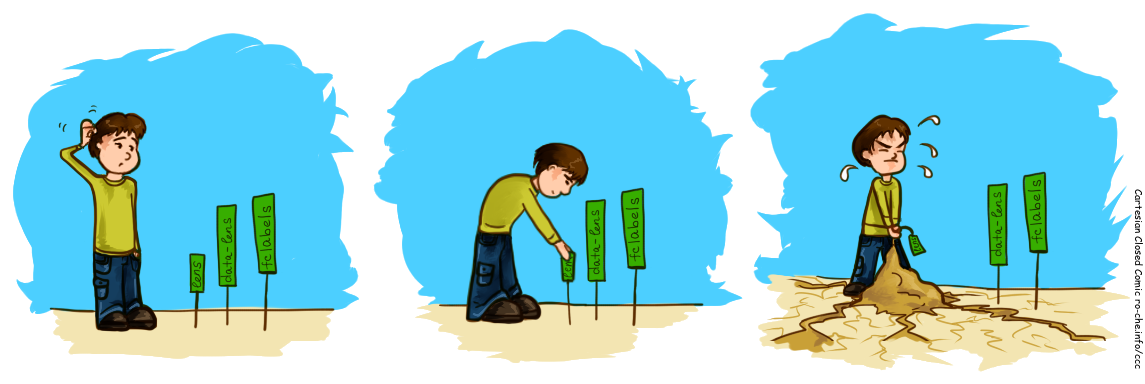
\includegraphics[width=0.9\linewidth]{ccc-picking-lens-library.png}
    \caption{Picking a Lens Library (Cartesian Closed Comic)}
  \end{figure}
\end{frame}

\end{document}
